% Quick start guide
\documentclass{beamer}
\usepackage{graphicx}%to use figures
\usepackage[font=small,labelfont=bf]{caption} %for captions of figures
\usepackage{pifont} %for the hand emphasis icon in lists
\usepackage{MnSymbol}
\usepackage{amsmath}
\usepackage{amssymb}
\usepackage{amsbsy}
\usepackage{tikz}
\usepackage{float}
\usepackage{listings}
\usetikzlibrary{decorations.text}
\usepackage{adjustbox}
\usepackage{booktabs}
\usepackage{multirow}
\usepackage{pgfgantt}
\usepackage{pgfpages}
\usepackage{enumerate}
\setbeameroption{show notes on second screen=right}
%\setbeameroption{show only notes}

\newcommand\blfootnote[1]{%
  \begingroup
  \renewcommand\thefootnote{}\footnote{#1}%
  \addtocounter{footnote}{-1}%
  \endgroup
}


%\usetikzlibrary{external}
%\tikzexternalize 
%load options
\usetikzlibrary{positioning,
calc,
shapes.geometric,
shapes.multipart,
shapes,
arrows.meta,
arrows,
decorations.markings,
trees}

%Create custom arrow style:
\tikzstyle{Arrow} = [
thick,
decoration={
markings,
mark=at position 0.999 with {
\arrow[thick]{latex}
}
},
shorten >= 3pt, preaction = {decorate}
]
\tikzstyle{Arrow2} = [
thick,
decoration={
markings,
mark=at position 0.999 with {
\arrow[thick]{latex}
}
},
shorten <-> 3pt, preaction = {decorate}
]
\usetheme{UNCMath}
\setbeamersize{text margin left=5mm,text margin right=5mm} 

% Title page details
\title[SER 2024: Improving Inferences from RCTs]{Improving Inferences from Randomized Trials:\\ 
Using per-protocol analyses obtain better estimated of HIV treatment effects.}

\author[Timothy Feeney]{by Timothy Feeney \\
SER June 19 2024}
%\institute[UNC-Chapel Hill]{Gillings School of Global Public Health; UNC-Chapel Hill}
\date{e: feeney@unc.edu, bsky: @tfeend.bsky.social}
\titlegraphic{
\includegraphics[width=\textwidth]{images/gillings_blue.jpg}}
\begin{document}


\begin{frame}
% Print the title page as the first slide
    \titlepage
\end{frame}


\begin{frame}{Outline}
            \tableofcontents
    \note{Today I will be working with other presenters to both explain how per-protocol analyses can facilitate better estimates and also convince you that this is the way forward.\\
    \vspace*{.5cm} 
    Ill start with background about RCTs, define per protocol effects, and then finish up with an example.}
\end{frame}

\section{RCTs}
    \begin{frame}{Randomized Trials are a gold standard}
        \begin{itemize}
            \item Require clear enrollment criteria
            \item Unabmiguous intervention protocol
            \item Exchangeability: $Y^a \upmodels A $ \hspace{0.5cm}for $A \in \{0,1\}$  
            \item Consistency: $Y=Y^{a=1}A+Y^{a=0}(1-A)$
            \item Positivity\footnotemark[1]: $Pr(A=a)>0$, $\forall \mathbf{\ell}$ where $f(a)>0$
            \item[\ding{43}] This allows for unbiased estimation of treatment effects.
        \end{itemize}
        \footnotetext[1]{$\mathbf{L}$ is covariate vector}  
        \note{\begin{itemize}
        \item RCTs are classically considered the gold standard in evaluating treatment effects. The status of RCTs originates from aspects of the design that help assure causal estimates are identified
        \item Some of these included clear enumeration of the population unders study, clearly laid out treatment protocols, and other causal identification criteria of marginal exchangeability, causal consistency and positivity being met by design.
    \end{itemize}} 
    \end{frame}

    \begin{frame}{RCT estimands}
        \begin{itemize}
            \item Intention-to-treat (ITT) effect: $E[Y^{r=1}]-E[Y^{r=0}]$
            \item This is the effect of treatment assignment on outcomes
            \item Public health focused
            \vspace{1cm}
            \item \textit{Typical} Per-protocol (PP) effect: $E[Y^{r=1, \bar{a}=1}]-E[Y^{r=0, \bar{a}=0}]$
            \item This is the effect of treatment assignment and adherence on outcomes
            \item Patient focused\footnotemark[1]
        \end{itemize}
        \blfootnote{$r =$ randomization; $\bar{a}=$ history of treatment adherence} 
        \footnotetext[1]{Hernan and Robins, NEJM 2016}
        \note{
        \begin{itemize}
        \item There are two commonly reported estimands in an RCT. The primary result reported is typically the intention-to-treat results which present the outcomes had everyone been assigned to treatment 1 versus everyone being assigned to treatment 0. 
        \item However, while this is public health focused, it is limited to evaluating the effect of randomization and not the effect of treatment.
        \item Instead, decision makers (e.g. physician) and those on the receiving end of the treatment may want to know instead waht is the effect if adherent to the treatment assignment. This cannot be answered with the ITT estimand and instead requires a per-protocol analysis that takes into account deviation or loss to follow up.
    \end{itemize}}
    \end{frame}

    \begin{frame}{Per-protocol effects can be biased}
        \begin{columns}
            \begin{column}{0.4\textwidth} 
        \begin{itemize}
            \item Frequently done by excluding those not adhering\footnotemark[1]
            \item Susceptible to selection bias
            \item[\ding{43}] Can be addresed: e.g with inverse probability weighting (see next talk) 
        \end{itemize}
    \end{column}

    \begin{column}{0.6\textwidth}   
         \begin{center}
            \resizebox{\textwidth}{!}{% 
        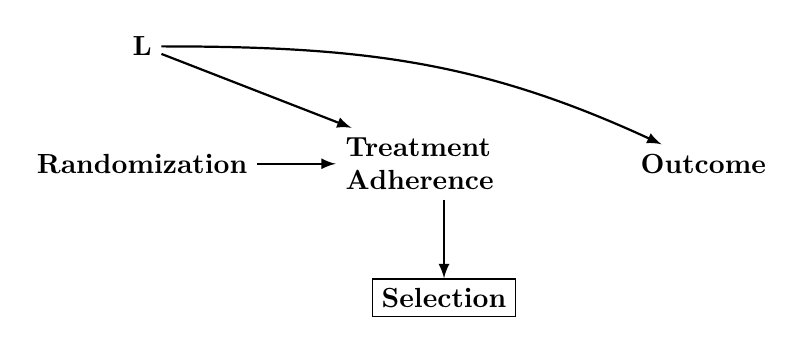
\begin{tikzpicture}
            \node (1) {\textbf{Randomization}};
            \node [right =of 1, text width=2.5cm] (2) {\textbf{Treatment Adherence}};
            \node [right =of 2] (3)  {\textbf{Outcome}};
            \node [above =of 1] (5) {$\mathbf{L}$};
            \node [rectangle, draw, below =of 2] (6){\textbf{Selection}};
            
            \draw[Arrow] (1) to (2);
            \draw[Arrow] (5) to (2);
            \draw[Arrow] (5) to [out=0, in=155] (3);
            \draw[Arrow] (2) to (6);
        \end{tikzpicture}
            }
    \end{center}
    \end{column}
\end{columns}
\footnotetext[1]{Cole \textit{et al.} JAMA Net. Open 2023, Dodd \textit{et al.} Trials 2012}
\footnotetext{$\mathbf{L}$ : vector of covariates} 
    \note{
        \begin{itemize}
            \item Per protocol effects are typically estimated by excluding those that deviate from the protocol
            \item However, these estimates should be thought of more like analyzing an observational study where common causes of the outcome of interest and adherence should be accounted for--this has been well reported since 2001 by Robins and Finkelstein
            \item As a result of this per protocol estimates can be biased.
            \item Here is a simple DAG illustrating the problem. If per protocol analyses are done where only those who adhere are included you create a selection bias. 
            \item Here this is by conditioning on a selection which is downstream of a collider, treatment adherence.
            \item However instead of restricting to only those that adhere there are ways around this which will be covered by the other speakers.
        \end{itemize} 
    }
    \end{frame}

  
\section{Per-protocol effects}
    \begin{frame}{There is no \textit{one} per-protocol effect}
        % \begin{columns}
        % \begin{column}{0.6\textwidth}
            \begin{itemize}
                \item Accounts for adherence
                \item "Doc, what if I take all my doses like you tell me to?"
                \item There are \textit{at least} 6 per-protocol parameters that can be estimated\footnotemark[1]
                \item There are also $k\in\{1,\ldots,\infty\}$ protocols depending on how the investigator(s) define adherence.
            \end{itemize}
        % \end{column}
        % \begin{column}{0.4\textwidth}
        %     $$
        %     \begin{aligned}
        %     & E\left[Y^{r=1, \bar{a}=1}\right]-E\left[Y^{r=0, \bar{a}=1}\right] \\
        %     & E\left[Y^{r=1, \bar{a}=1}\right]-E\left[Y^{r=0, \bar{a}=0}\right] \\
        %     & E\left[Y^{r=0, \bar{a}=1}\right]-E\left[Y^{r=0, \bar{a}=0}\right] \\
        %     & E\left[Y^{r=1, \bar{a}=1}\right]-E\left[Y^{r=1, \bar{a}=0}\right] \\
        %     & E\left[Y^{r=0, \bar{a}=1}\right]-E\left[Y^{r=1, \bar{a}=0}\right] \\
        %     & E\left[Y^{r=1, \bar{a}=0}\right]-E\left[Y^{r=0, \bar{a}=0}\right]
        %     \end{aligned}
        %     $$
        % \end{column}
        % \end{columns}
        \footnotetext[1]{Rudolph \textit{et al.} Epidemiology 2020}
        \note{However there is no ONE per protocol effect and there are at least 6 estimands that can be considered per protocol effect. They are llustrated here.
        \begin{itemize}
            \item For instance if you look at the second line this answers "what if I took my treatment as assigned the whole way through the trial" where as line five asks "what if I did the opposite of what I was assigned the whole way through the trial?"
            \item These estimands can be made even more precise to account for deviating from 1 to many doses--more on this in a bit.  
        \end{itemize}
       }
    \end{frame}
       
   
  
    \begin{frame}{Per Protocol Causal Identification}
        \begin{itemize}
            \item Conditional Exchangeability: $Y^g \upmodels \left(A_t,C_{t+1}\right) \mid \left(\bar{A}_{t-1}=\bar{a}^g_{t-1}, \bar{L_t}=\bar{\ell_t}, C_t=Y_t=0\right)$ \hspace{0.25cm} $ \forall t$\vspace{1em}
            \item Consistency: if $\bar{A}_{t}=\bar{A}^g_{t}$ then $ \bar{Y}_t=\bar{Y}^g_t$\vspace{1em}
            \item Positivity:$f(a^g_t, C_t=0\mid\bar{a}^g_t,\bar{\ell}_t,C_t=Y_t=0)>0$ where $f(\bar{a}^g_t,\bar{\ell}_t, C_t=Y_t=0)>0$ \hspace{0.25cm} $ \forall t$\vspace{1em}
            \item No interference:$\bar{A}^g_{it} \upmodels \bar{Y}^g_{jt}$ where $i \ne j$
            \item No missclassification and correct model specification 
        \end{itemize}
        \vspace{0.5cm}
        $Y=$outcome, $C$=censoring, $A=$ treatment , $L=$ covariates, $t$ =time point from $0 \ldots t$, $g$ is a deterministic treatment strategy, overbar denotes history of values
        \footnotetext{Wen \textit{et al.} Biometrics 2019}
        \note{The causal idenfication criteria are slightly modified to account for the treatment regimens described by the trial protocol. This allows for us to take time into account
            \begin{itemize}
                \item now we assume that adherence and censoring is independent of an individuals counterfacutal outcome conditional on adherence under a specific treatment regimen at all prior times,and covariate values at all time points
                \item Consistency is now that your counterfactual outcome for a treatment regimen is the outcome observed under that treatment regimen
                \item Positivity requires nonzero joint probability of treatment adherence and being uncensored at each time point conditional on covariates
                \item No interference at each time point.
                \item and of course no missclassification or model misspecification

            \end{itemize}
        }
        \end{frame}

% \begin{frame}{More on Protocol Definition}
% \centering
% \begin{tikzpicture}
%     % Draw x and y axis
%     \draw[-] (0,0) -- (5.3,0) ; % Draw x-axis up to 5
%     \draw[->] (0,0) -- (0,6) node[above] {Protocols};

%     % Draw x axis labels
%     \foreach \x in {1,2,...,5}
%         \draw (\x,0.1) -- (\x,-0.1) node[below] {\x};

%     % Draw y axis labels
%     \foreach \y in {5,4,...,1}
%         \draw (-0.1,\y) -- (0.1,\y) node[left] {\y};

%     % Draw lines for individuals
%     \draw (0,1) -- (5,1);
%     \draw (0,2) -- (4,2);
%     \draw (0,3) -- (3,3);
%     \draw (0,4) -- (2,4);
%     \draw (0,5) -- (1,5);

%     % Draw censor marks 
%     \node at (1,5) {$>$};
%     \node at (2,4) {$>$};
%     \node at (3,3) {$>$};
%     \node at (4,2) {$>$};
%     \node at (5,1) {$>$};

%     % Add a small discontinuity on the x axis
%     \draw[thick] (5.3,0.1) -- (5.4,-0.1);
%     \draw[thick] (5.4,0.1) -- (5.5,-0.1);

%     % Draw the rest of the x-axis with a gap
%     \draw[->] (5.5,0) -- (6.5,0);

%     % Add infinity symbol on the x axis
%     \node at (7.3, 0) {$\infty$ Doses};
%     \node at (6, -0.4) {};
%     \node at (3.5, -1) {Doses allowed};
% \end{tikzpicture}
% \note{
%     \begin{itemize}
%         \item Before I mentioned that there is both no one protocol, but also that this definition can be modulated; This figure attempts to illustrate this point.
%         \item On the x-axis there are the number of doses allowed before the protocol has been violated and censoring occurs. The ITT analysis would be infinite number of doses, becuase the only thing that matters is randomization assignment.
%         \item Person one is allowed to miss 4 doses and on the 5th missed dose or treatment they are censored. Other protocols are still possible, for instance protocol 2 only allows 3 missed doses and porotocl 5 allows none, and a participant is censored as soon as they miss one dose.
%         \item We will use this approach in the example I will highlight next
%     \end{itemize}
% }
% \end{frame}

\section{Example using ACTG 5202 Trial}

\begin{frame}
    \huge
    \centering
    An example using an HIV Trial: \\
   
    AIDS Clinical Trial Group (ACTG) 5202
    \note{ Ill now go over some results from a per protocol analysis that varies how protocol is defined in order to illustrate my point.}
\end{frame}

\begin{frame}{Role of adherence in HIV treatment efficacy}
    \begin{columns}
    \begin{column}{0.45\textwidth}
        \begin{itemize}
            \item Adherence needed for HIV viral suppression varies by treatment regimen.
            \item Blanket recommendations fail.
            \item[\ding{43}] Understanding of how adherence impacts efficacy is \textit{critical}\footnotemark[1] for:
            \begin{itemize}
                \item Developing new treatments.
                \item Maximizing current treatments.
            \end{itemize}
        \end{itemize}
        \footnotetext[1]{\tiny Adimora, Cole and Eron CID 2017}
    \end{column}
% Column 2
    \begin{column}{0.55\textwidth}
    \begin{figure}
        \centering
        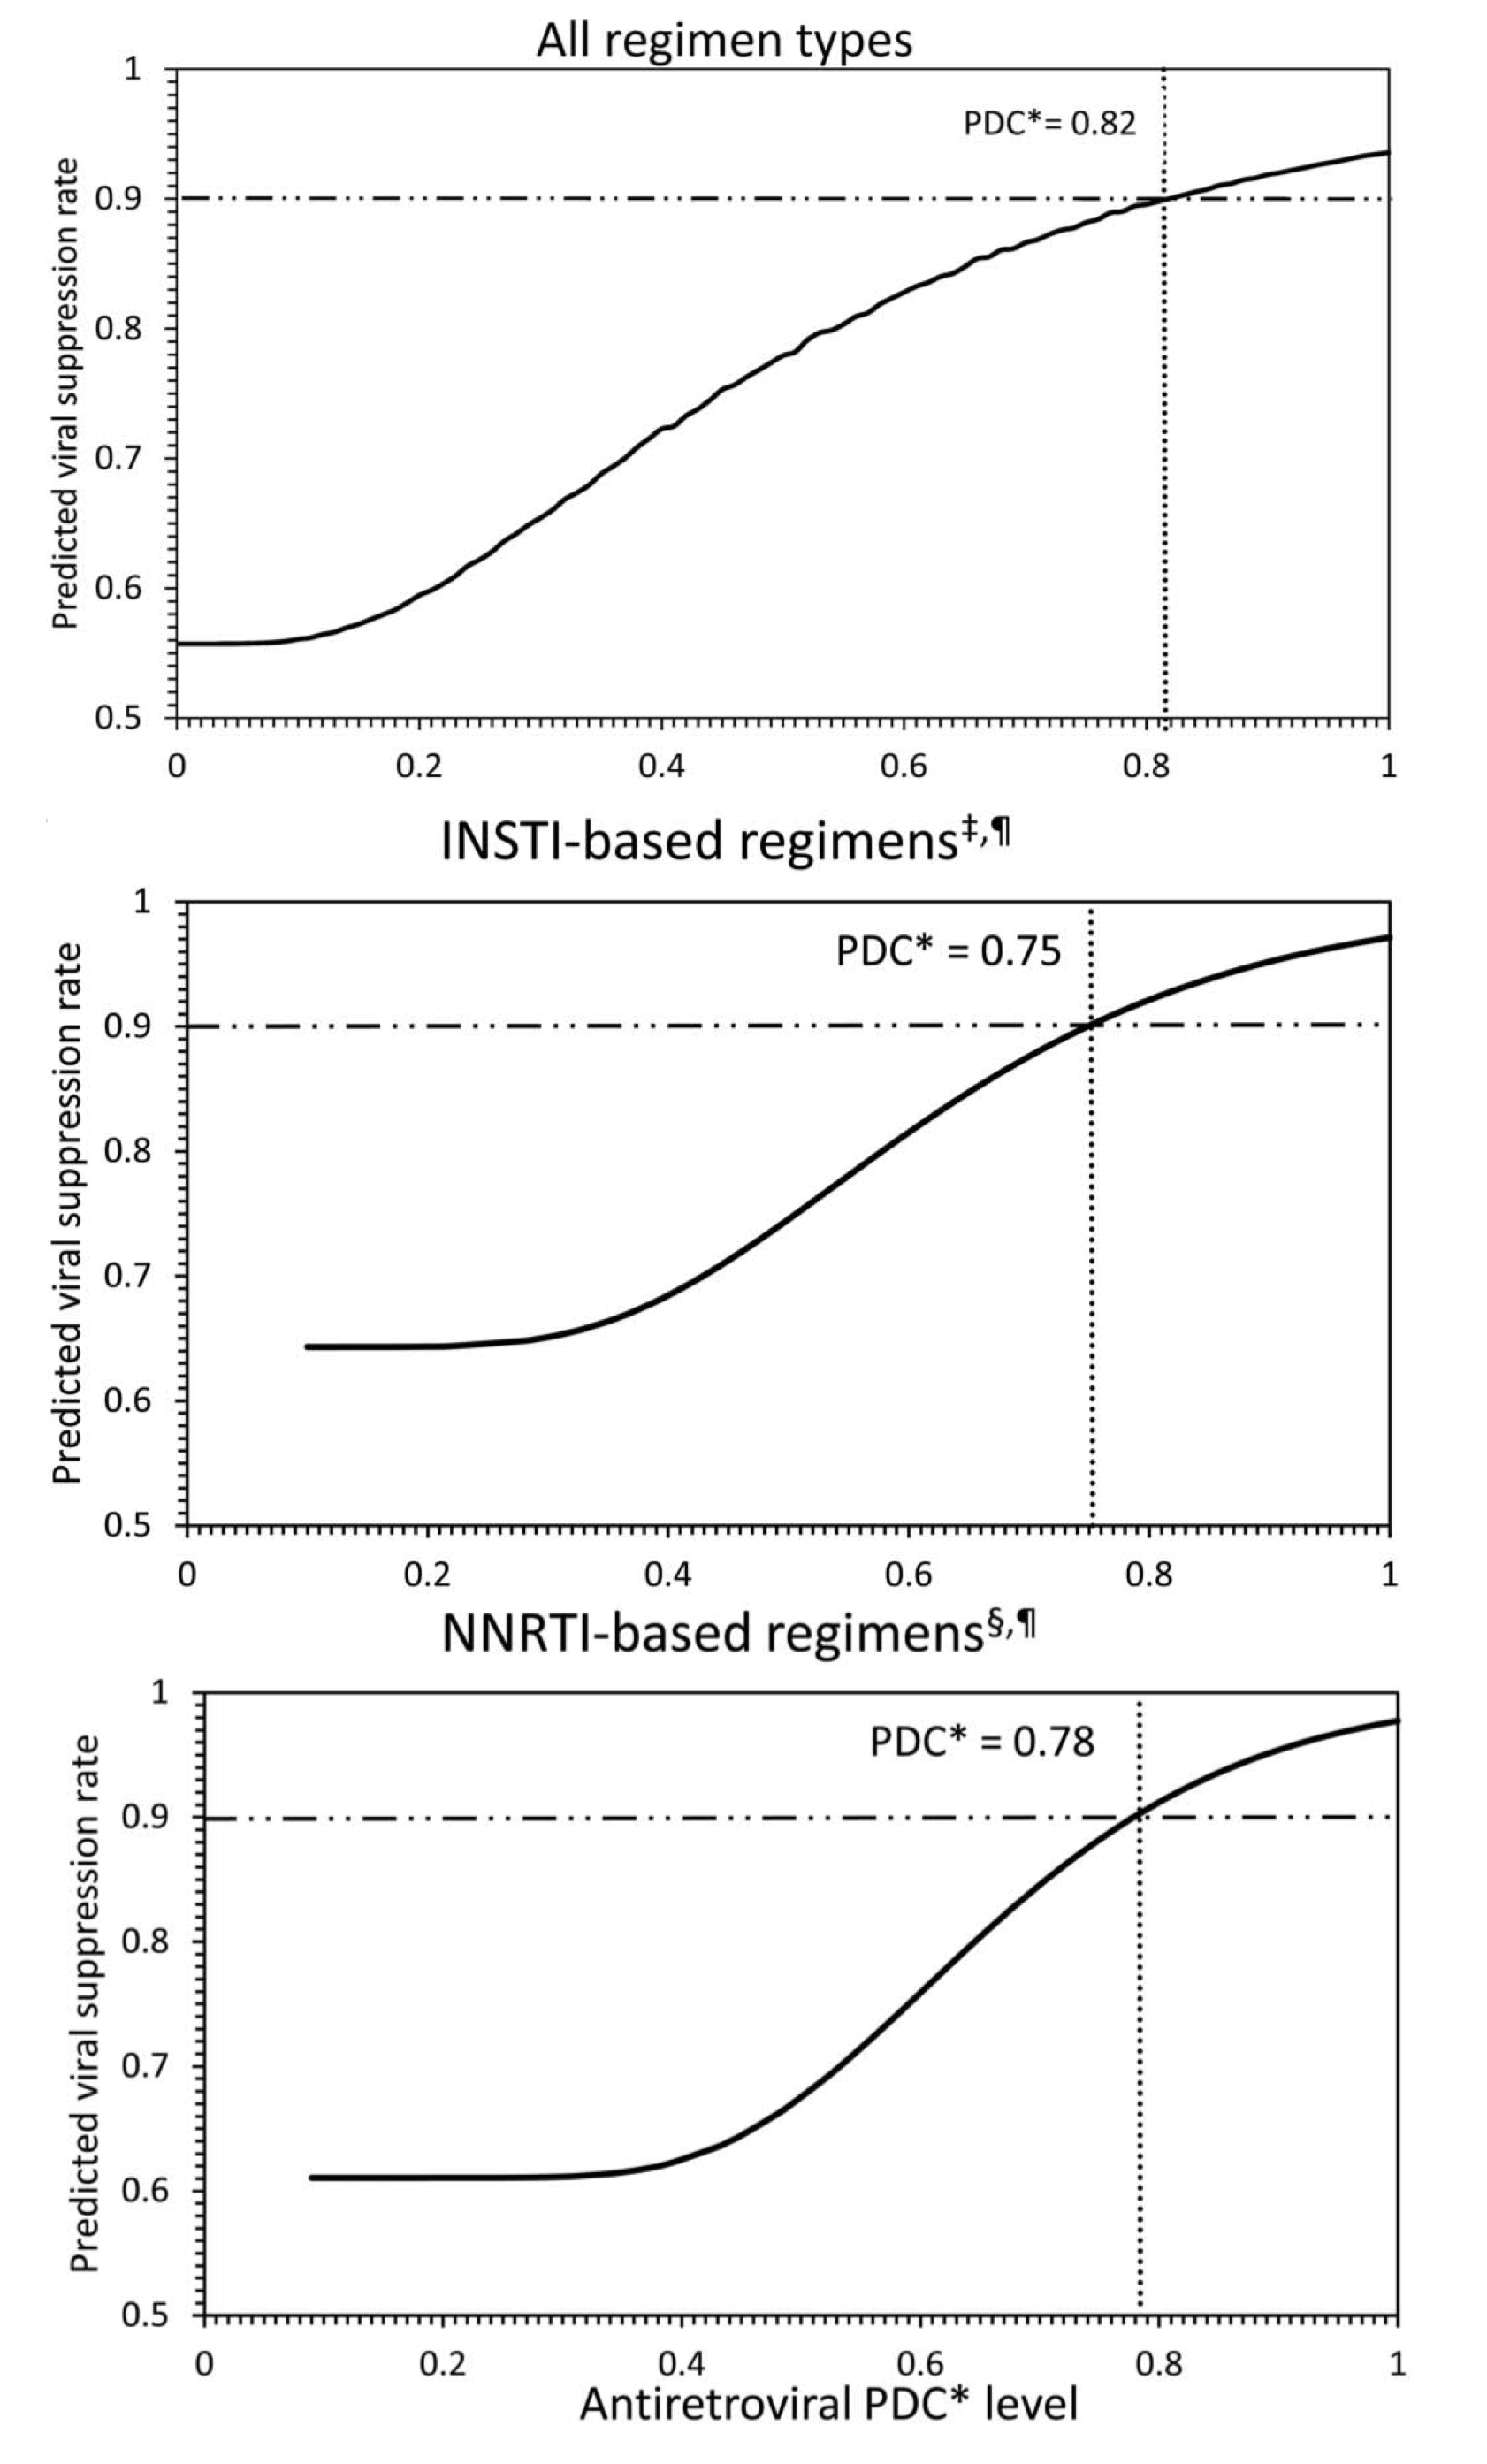
\includegraphics[scale=0.0750]{figs/fig2.png}
        \caption*{}
        \label{fig:fig2}
    \end{figure}
    \end{column}
\end{columns}

\note{The efficacy of HIV treatments depends both on the mechanism of the medication and the adherence to a dosing scheme. In general it is not possible to make a blanket statement that any number of missed doses per time-frame is ok or not. Thus evaluating adherence in in terms of doses taken should be considered.} 
\end{frame}   

    \subsection{Population}


\begin{frame}{ACTG 5202 Study Population}
    Phase 3b RCT at 59 sites, US and Puerto Rico
    \vspace{0.53cm}

    \resizebox{\textwidth}{!}{% 
    \begin{tabular}{lll}
         & ABC/3TC & TDF/FTC\\
        \midrule
        N & 928 & 929\\
        \addlinespace[0.1cm]\\
        Male at birth \% & 81.4 & 84.0\\
        \addlinespace[0.1cm]
        Age Group \% & & \\
        \quad$\leq25$& 10.1 & 10.5\\
        \quad 26-49& 77.0& 74.8\\
        \quad$\geq50$ & 12.8 &14.6\\
        \addlinespace[0.1cm]
        Baseline log$_{10}$ RNA copies/mL(med [IQR]) & 4.66 [4.31, 5.06] & 4.65 [4.34, 4.96]\\
        \addlinespace[0.1cm]
        Baseline CD4 count/mL (med [IQR]) & 229 [84, 338] & 230 [97, 330]\\
        \addlinespace[0.1cm]
        \bottomrule
        \end{tabular}
    }
    \note{Phase 3 RCT in 59 sites in the US and Puerto Rico participants Randomized 1:1  TDF/FTC or ABC/3TC
  
    \begin{itemize} 
        \item TDF/FTC + (EFV or ATV/r) + ABC/3TC placebo
        \item ABC/3TC + (EFV or ATV/r) + TDF/FTC placebo
        \item Stratified by HIV-1 RNA screening level of
        \item $< 100,000$
        \item or  $\geq 100,000$ 
    \end{itemize}}
\end{frame}

    \begin{frame}{Example: ACTG 5202 Reanalysis}
            Objective:
        \begin{itemize}
            \item Estimand: $E\left[Y^{r=1,\bar{a}=1}\right]-E\left[Y^{r=0,\bar{a}=0}\right]$ at 48 weeks %and 96 weeks.
            \item Per-protocol analyses modulating $\bar{a}$.
            \item Protocol will depend on number of doses missed
        \end{itemize}
        \vspace{0.5cm}
        Outcomes: Composite virologic failure and all-cause mortality:
        \note{The ACTG 5202 study was a phase 3 trial throughout the US and Puerto Rico. The findings were published in 2009 and then in 2011
        \begin{itemize}
            \item We reanalyzed this data with the goal to evaluate treatment effects in under multiple protocol definitions to estimate treatment efficacy in the population of HIV+ person in the United states. 
            \item We aimed to estimate the risk difference at 48 weeks %and 96 weeks. 
        \end{itemize}
        }
    \end{frame}

\subsection{Analysis Plan}

\begin{frame}{DAG}
    \begin{figure}
    \centering
       \resizebox{0.95\textwidth}{!}{
           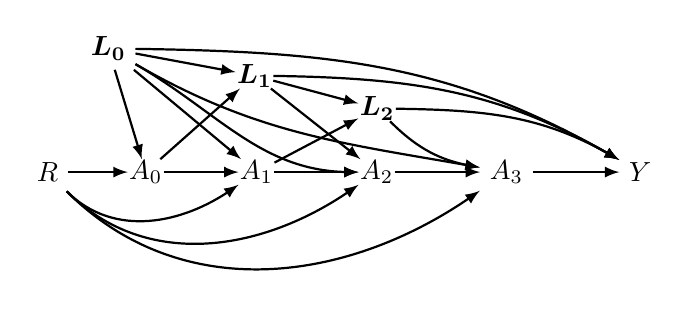
\begin{tikzpicture}
   \node [inner sep=0.1mm](a0) at (-3.281,0.386) {${A_0}$};
   \node [inner sep=0.1mm](a1) at (-1.874,0.386) {$A_1$};
   \node[inner sep=0.1mm] (a2) at (-0.348,0.386) {$A_2$};
   \node (l0) at (-3.757,1.956) {$\boldsymbol{L_0}$};
   \node[inner sep=0.1mm] (l1) at (-1.900,1.611) {$\boldsymbol{L_1}$};
   \node [inner sep=0.1mm] (l2) at (-0.342, 1.194) {$\boldsymbol{L_2}$};
    \node (r) at (-4.529,0.386) {$R$};
    \node (a3) at (1.3,0.386) {$A_3$};
     \node (y2) at (3,0.386) {$Y$};

   \draw [Arrow] (r) to (a0);
   \draw [Arrow] (a0) to (a1);
   \draw [Arrow] (a1) to (a2);
   \draw [Arrow] (a2) to (a3);
   \draw [Arrow] (a3) to (y2);
   \draw [Arrow] (l0) to (a0);
   \draw [Arrow] (l0) to (a1);
   \draw [Arrow] (l1) to  (a2);
   \draw [Arrow](l2) to [out=-45, in=170] (a3);
   \draw [Arrow](l0) to (l1);
   \draw [Arrow] (l1) to (l2);
   \draw [Arrow] (a0) to (l1);
   \draw [Arrow] (a1) to (l2);
    \draw[Arrow] (l0) to [out=-0.956, in=150] (y2);
    \draw[Arrow] (l1) to [out=-0.956, in=150] (y2);
    \draw[Arrow] (l2) to [out=-0.956, in=150] (y2);
    \draw[Arrow] (l0) to [ out=-30, in=180] (a2);
    \draw[Arrow] (l0) to [ out=-30, in=170] (a3);
    \draw[Arrow] (r) to [out=-45, in=-145] (a1);
    \draw[Arrow] (r) to [out=-45, in=-145] (a2);
    \draw[Arrow] (r) to [out=-45, in=-145] (a3);
\end{tikzpicture}
           }
       \label{fig:aim2-dag}
       \end{figure}
$j$: follow up time, $\mathbf{L_j}$: vector of covariates at follow up time $j$\\

$A_j$: tx adherence at follow up time $j$, $R$: randomization, $Y$: viral failure or death       
\note{A simplified DAG illustrates our assumptions. We are assuming that randomization to treatment impacts adherence, and that baseline covariate values and covariate values at the preceeding time point also impacts adherence and the outcome.\\
\vspace{0.5cm}
we will use IPW in the analysis here to account for these factors that leads to differences in adherence and the outcome} 
   \end{frame}

\begin{frame}{Adherence and Protocol}
Adherence evaluated in-person at 8, 24, 48, 72, 96, then every 24 weeks and either at the final study evaluation or after virologic failure.

\begin{table}
\centering
\resizebox{0.5\textwidth}{!}{
\begin{tabular}{p{4cm} p{4cm}}
\toprule
\textbf{Last Time Missed Medication} & \textbf{How Close Was Dose Schedule Followed} \\
\midrule
Never & Never \\
$>$3 months ago & Some of the time \\
1-3 months ago & About half the time \\
2-4 weeks ago & Most of the time \\
1-2 weeks ago & All the time \\
Within the past week & \\
\bottomrule
\end{tabular}
}
\end{table}

\begin{table}[htbp]
\centering
\resizebox{\textwidth}{!}{
\begin{tabular}{ll}
    \hline
    \textbf{Protocol Definition} & \textbf{Description of Protocol} \\

    0 dose missed OK & No report of missed medication doses \\

    1 dose missed OK & Participant with only one report of missed medication doses \\

    \vdots & \vdots \\
    4 doses missed OK & Participant with $\geq 10$ reported missed medication doses without overlap in reported timing \\
    \hline
\end{tabular}
}
\end{table}
\note{Adhrence in ACTG 5202 was collecetd by self report and whether or not there were missed doses within a previous time frame. There was also information about how closesly a dosing regimen was followed but we did not incorporate that here.\\
\vspace{0.5cm}
We defined protocol deviation, illustrated in the bottom table,  by how many missed doses were acceptable. For instance if 0 doses missed were OK, then as soon as a person reported missing any doses they were censored. For those where missing 4 doses was ok, as soon as they missed the fifth dose they were censored.} 
\end{frame}


\subsection{Results}

\begin{frame}{Deviation from Defined Protocols}
    \centering
    \resizebox{\textwidth}{!}{%
    \begin{tabular}{llllllll}
        \toprule
        Treatment Group & Censored & 1 Dose & 2 Dose & 3 Dose & 4 Dose & 5 Dose & Total\\
        \midrule
        ABC/3TC & 234 & 276 & 110 & 57 & 18 & 7 & 928\\
        TDF/FTC & 211 & 263 & 79 & 38 & 23 & 7 & 929\\
        \bottomrule
        \end{tabular}
    }
    \note{As might be expected as the definition of protocol deviation becomes more strict, requiring more missed doses to be censored, there is a decrease in the number of participants deviating from the protocol. This goes from 276 in the ABC arm and 263 in the TDF arm for the 1 dose protocol down to 7 in each arm under the 5 dose protocol definition.}
\end{frame}



\begin{frame}
    \begin{figure}[H] 
        \centering
        \includegraphics[width=\textwidth]{/Users/timf/Library/CloudStorage/OneDrive-UniversityofNorthCarolinaatChapelHill/Dissertation/DissertationAnalysis/Aim 2/results/figures/ser_surv1.png} 

        \caption*{} 
        \label{fig:mutli_surv} % Add a label for referencing the figure
    \end{figure}
    \note{now we turn our attention to the risk of viral failure and death. There are two notable findings here. 
    \begin{enumerate}
        \item the absolute risk of an outcome in both arms under the 1 dose missed protocol is lower suggesting higher risk people are missing 1 dose of medication. 
        \item There is a smaller difference in the risk when accounting for 1 dose protocol deviation. This is a bit harder to see here, but will become a little more apparent on the next slide.
    \end{enumerate}}
\end{frame}

\begin{frame}
    \begin{figure}[H] 
        \centering
        \includegraphics[width=\textwidth]{/Users/timf/Library/CloudStorage/OneDrive-UniversityofNorthCarolinaatChapelHill/Dissertation/DissertationAnalysis/Aim 2/results/figures/ser_surv2.png} 

        \caption*{} 
        \label{fig:mutli_surv} % Add a label for referencing the figure
    \end{figure}
    \note{now we turn our attention to the risk of viral failure and death. There are two notable findings here. 
    \begin{enumerate}
        \item the absolute risk of an outcome in both arms under the 1 dose missed protocol is lower suggesting higher risk people are missing 1 dose of medication. 
        \item There is a smaller difference in the risk when accounting for 1 dose protocol deviation. This is a bit harder to see here, but will become a little more apparent on the next slide.
    \end{enumerate}}
\end{frame}


\begin{frame}
     \begin{figure}[H] 
           \centering
            \includegraphics[width=0.95\textwidth]{/Users/timf/Library/CloudStorage/OneDrive-UniversityofNorthCarolinaatChapelHill/Dissertation/DissertationAnalysis/Aim 2/results/figures/tvary_wk48_forest.png} 
            \caption*{} 
            \label{fig:48wk_forest} % Add a label for referencing the figure
     \end{figure}
     \note{here we can see the risk differences and 95\% confidence intervals based on robust standard errors. As expected as we censored individuals the standard error increased. The changes in the risk difference become more apparent with smaller risk differences when accounting for 1 and 2 dose deviations. This suggest the efficacy of the TDF versus ABC is not quite as large as you might expect if you relied only on a naive analysis.} 
\end{frame}

% \begin{frame}
%     \begin{figure}[H] 
%         \centering
%         \includegraphics[width=0.95\textwidth]{/Users/timf/Library/CloudStorage/OneDrive-UniversityofNorthCarolinaatChapelHill/Dissertation/DissertationAnalysis/Aim 2/results/figures/tvary_wk96_forest.png} 
%         \caption*{} 
%         \label{fig:96wk_forest} % Add a label for referencing the figure
%     \end{figure}  
% \end{frame}
    
 
 \subsection{Limitations and Future}
    
    \begin{frame}{Limitations and Future Plans}

    \begin{enumerate}
        \item Completed with public access data\footnotemark[1]
        \item Reliance on coarse, self-reported medication adherence
        \item Assume identification conditions met.\footnotemark[2]
        \item Future directions include repeating analysis with g-formula, considering additional protocols. 
    \end{enumerate}
\footnotetext[1]{Approved for more granular data from ACTG, awaiting dataset}
\footnotetext[2]{NB: not guaranteed in per-protocol setting even though it is a trial}
\note{This is a work in progress and There were some limitations.
\begin{enumerate}
    \item this analysis was completed with public data. We have approval from ACTG to obtain more granular data and we will update our results with that
    \item currently this analysis relied on coarse data on adherence and I am currently working to improved estimates of the number of doses that people actually missed.
    \item we assume that we have met all the required identification condigions based on covariates in the IPW models.
\end{enumerate}
Our future directions are to also complete this analysis using the g-formula, and also consider additional granular data once the ACTG provides us with an updated data set}
    \end{frame}

 \section{Closing Remarks}
\begin{frame}{Takeaways}
\begin{itemize}
\item Per protocol analysis should be treated like an observational analysis.
\item Time varying analysis needs to be accounted for.
\item There are many ways protocols can be defined.
\item The way protocol is defined can have meaningful impacts on estimates.
\end{itemize}

\end{frame}

    
 \begin{frame}
    {\Huge Thank you!}
    \begin{figure}[H] 
       \centering
        
\includegraphics[width=\textwidth]{images/gillings_blue.jpg} 
       \caption*{} 
   \end{figure}  
       
       \begin{columns}
        \begin{column}{0.5\textwidth}
             I'd like to acknowledge:
             \begin{itemize}
                \item Steve Cole
                \item Paul Zivich
                \item Catherine Li
                \item ACTG 5202
                \item ACTG 5202 Particpants
                \item Cole Lab Members
             \end{itemize}
        \end{column}
        \begin{column}{0.5\textwidth}
           
           \begin{figure}[H] 
               \centering
               
\includegraphics[width=0.5\textwidth]{images/qr_black.png} 
               \caption*{My website where you can find a link to my github.} 
           \end{figure} 
       \end{column} 
        
     \end{columns}
     \note{Thank you for your time. Id like to acknowledge the Steve Cole, the cole lab, Paul Zivich, Catherine Li and all the participants of the ACTG 5202 study whom without their participation this work would not be possible.} 
\end{frame}

\section*{Appendix}
\begin{frame}{Outcome Definition}
 \begin{itemize}
         \item plasma HIV-1 RNA level $\geq$1000 copies /mL between 16 weeks and 24 weeks
         \item or $\geq$200 copies/mL at or after 24 weeks
         \item  all cause mortality
        \end{itemize} 
\end{frame}

\begin{frame}{Censoring Risk}
    \begin{figure}[H] 
        \centering
        \includegraphics[width=\textwidth]{/Users/timf/Library/CloudStorage/OneDrive-UniversityofNorthCarolinaatChapelHill/Dissertation/DissertationAnalysis/Aim 2/results/figures/tvary_censor_surv.png} 

        \caption*{} 
        \label{fig:cens_surv} % Add a label for referencing the figure
    \end{figure}
\note{here are risk curves for censoring and censoring +protocol deviation. The black line shows only the risk for loss to follow up and there is little difference between the two arms. The red line shows a similar pattern that overlaps closely with the censoring arm. We would expect the more doses required to be missed to approximate the censoring arm. However, if you look at the yellow line the overall risk of being censorid is higher and there is a slightly higher risk in the ABC arm versus the TDF arm in the later time points.}
\end{frame}


\end{document}